\documentclass[]{article}
\usepackage{graphicx, float}
\usepackage{hyperref}
%opening
\title{\centering CSP780 : Computer Vision \\Assignment - 1\\Report}
\author{Sahil\\  2016UCS0008}

\begin{document}
	
	\maketitle	
	\section{Introduction}
	\large
	We are given with a noisy image and it is to be smoothed by applying various spatial filters.
	\begin{figure}[H]
		\centering
		\vspace{0pt}
		\includegraphics[width=400pt, height = 150pt, keepaspectratio]{../tiffney_pgm_gaussian_noise.jpg}
	\end{figure}
	
	The following filters of sizes 3x3, 5x5 and 7x7 are applied and the various outputs obtained have been observed : \\
	\begin{itemize}
		\item Low-Pass (Average Filter)
		\item Gaussian Filter
		\item Bilateral Filter
		\item Non-local means filter
	\end{itemize}
 	Also, BRISQUE scores are obtained to get the No-Reference Image Quality Assessment Score. They are shown in the table below:
 	
 	\begin{figure}[H]       
 			\centering
 			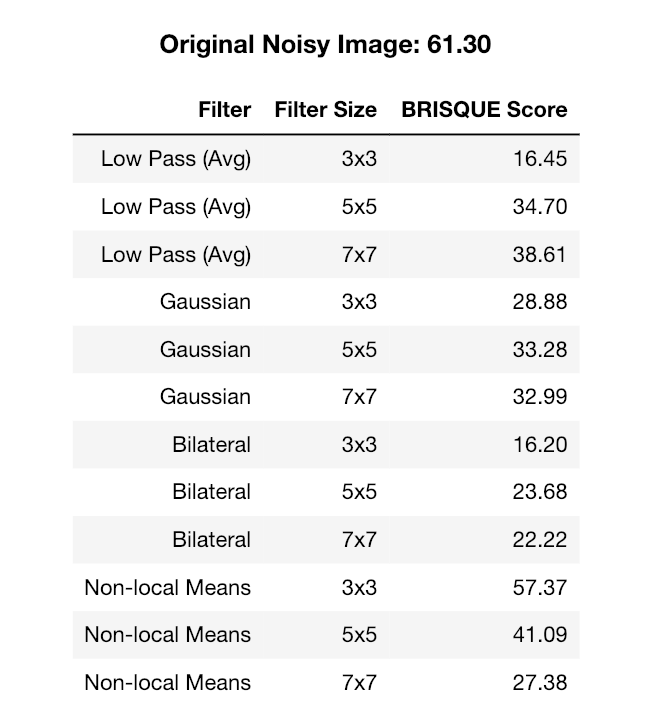
\includegraphics[width=800pt, height = 300pt, keepaspectratio]{./brisque_scores.png}  
 			\caption{Table showing the BRISQE scores}
 	\end{figure}
 	
 	From the table, we can draw the inference that the 3x3 bilateral filter gives the best perceptual quality image as it has the lowest BRISQUE score. Following this, the average 3x3 filter also provides a good image. 
 	
 	\section{Conclusion:}
 	- The bilateral filter includes both the qualities of the gaussian filter and also preserves the edges in the original image, thus reducing noise as well as maintaining image quality. \\
 	- The Gaussian filter does a better noise removal compared to the low pass average filter as visible from the BRISQUE scores. This is because the average filter leads to blurring effects. \\
 	- The non-local means 3x3 and 5x5 filtering has poor BRISQUE scores, which are closer to the noisy images. This is mainly due to the smaller filter size and larger 7x7 window considered. Also, NLM filtering is computationally complex, so other filtering techniques, being simple to compute are considered better. 
 	
 	
%	\begin{figure}[H]       
%		\centering
%		\includegraphics[width=400pt, height = 150pt, keepaspectratio]{../tiffney_pgm_gaussian_noise.jpg}  
%		\hspace{20px}
%		\includegraphics[width=400pt, height = 150pt, keepaspectratio]{../output_average3x3.png}
%		\hspace{20px}
%		\caption{Original image (left) vs Filtered image (Right) (\textbf{3x3 filter})}
%	\end{figure}
%
%	\begin{figure}[H]       
%		\centering
%		\includegraphics[width=400pt, height = 150pt, keepaspectratio]{../tiffney_pgm_gaussian_noise.jpg}  
%		\hspace{20px}
%		\includegraphics[width=400pt, height = 150pt, keepaspectratio]{../output_average5x5.png}
%		\hspace{20px}
%		\caption{Original image (left) vs Filtered image (Right) (\textbf{5x5 filter})}
%	\end{figure}
%
%	\begin{figure}[H]       
%		\centering
%		\includegraphics[width=400pt, height = 150pt, keepaspectratio]{../tiffney_pgm_gaussian_noise.jpg}  
%		\hspace{20px}
%		\includegraphics[width=400pt, height = 150pt, keepaspectratio]{../output_average7x7.png}
%		\hspace{20px}
%		\caption{Original image (left) vs Filtered image (Right) (\textbf{7x7 filter})}
%	\end{figure}

		

\end{document}
